%!TEX root = ../proyecto.tex
\chapter{Desarrollo de pruebas y análisis de resultados.}
\section{Entorno de pruebas.}
Para el desarrollo de las pruebas, mi ordenador personal ha sido utilizado. Las especificaciones ténicas relevantes del mismo son:

\begin{itemize}
\item \textbf{GPU}: \underline{Zotac GeForce GTX 1060 AMP! Edition.}
\end{itemize}

% Please add the following required packages to your document preamble:
% \usepackage{booktabs}
% \usepackage{longtable}
% Note: It may be necessary to compile the document several times to get a multi-page table to line up properly
\begin{longtable}{@{}lc@{}}
\toprule
\multicolumn{1}{c}{\textbf{Características}}     & \textbf{Valor}           \\* \midrule
\endfirsthead
%
\endhead
%
\bottomrule
\endfoot
%
\endlastfoot
%
\textbf{Núcleos CUDA}                            & 1290                     \\
\textbf{Frecuencia del procesador}               & 1771 MHz                 \\
\textbf{Frecuencia de la memoria}                & 4004 Mhz                 \\
\textbf{Memoria global total}                    & 6 GB DDR5                \\
\textbf{Bus de memoria}                          & 192-bit                  \\
\textbf{Compute Capability}                      & 6.1                      \\
\textbf{Número de hebras por bloque}             & 1024                     \\
\textbf{Dimensión máxima del bloque (x, y, z)}   & 1024, 1024, 64           \\
\textbf{Dimensión máxima del ``grid'' (x, y, z)} & 2147483647, 65535, 65535 \\
\textbf{Número de registros por bloque}          & 65536                    \\
\textbf{Memoria compartida por bloque}           & 49152 KB                 \\
\textbf{Número de multiprocesadores}             & 10                       \\
\textbf{Modelo de driver CUDA}                   & WDDM                     \\
\textbf{Versión del driver CUDA}                 & 417.35                   \\
\textbf{Versión del SDK CUDA}                    & 10.0                     \\* \bottomrule
\caption{Características de la GPU NVIDIA GeForce GTX 1060 6 GB}
\label{tab:esptec}\\
\end{longtable}

\begin{itemize}
	\item \textbf{Placa Base:} MSI B450M Bazooka.
	\item \textbf{Sistema Operativo:} Windows 10 Home 64 bits.
	\item \textbf{CPU:} AMD Ryzen 5 2600X.
	\item \textbf{RAM:} Kingston HyperX Fury Black DDR4 2400 MHz PC4-19200 8GB CL15.
\end{itemize}
\section{Conjuntos de datos utilizados.}

Durante la fase de desarrollo del mapa auto-organizado hemos utilizado el conjunto de datos de las \textbf{caras de Olivetti}, creado por \textit{AT\&T Laboratories Cambridge} y descargada a través del paquete de Python \textit{scikit-learn} \cite{olivetti}. Dicho conjunto de imágenes consiste en 400 imágenes de 40 sujetos en escala de grises. Cada muestra son los valores de intensidad de cada píxel con un valor normalizado entre 0 y 1. Además, se proporciona una etiqueta que indica a qué sujeto pertenece cada imagen, pero para los propósitos de nuestro modelo de aprendizaje no supervisado la misma no será utilizada. Las imágenes están en una versión cuadrada de 64x64 píxeles dándonos un total de 4096 valores de intensidad por muestra. \\


Para evaluar el rendimiento de ambos modelos para conjuntos de \textit{Big Data} hemos utilizado \textbf{SUSY} \cite{susy}. Este conjunto de datos contiene 5 millones de muestras con 18 atributos, que se generó a partir de un experimento de física en el que también se intenta diferenciar un proceso que genera partículas supersimétricas (\textit{signal}) de otro proceso que no las genera (\textit{background}). En el caso del mapa auto-organizado, la clase de salida es ignorada. De manera similar al anterior, los datos del conjunto fueron generados a partir de simulaciones de Monte Carlo.


\section{Experimentos para evaluar el mapa auto-organizado.}
\subsection{Verificación de la implementación del modelo.}
En el caso del mapa auto-organizado, tanto la versión como para CPU como para GPU ejecutan el mismo algoritmo, por lo que las métricas de interés durante las ejecuciones realizadas son el tiempo de ejecución y la ganancia. En primer lugar, durante la fase de desarrollo usamos el conjunto de las caras de \textit{Olivetti}, que nos permitió comprobar de manera empírica y visual que los resultados obtenidos por el algoritmo son son correctos. En caso de funcionar correctamente, obtendríamos un conjunto de imágenes con la misma dimensión del mapa de neuronas, que son o se parecen a algunas de las caras de los sujetos, y donde las imágenes más parecidas se encuentran próximas las unas con las otras. \\

Para este experimento, generamos un mapa de 5 filas y 6 columnas, y, ejecutamos el algoritmo durante 50 iteraciones, con 25 para la primera fase y otras 25 para la segunda fase y con los parámetros de control $\sigma_0, \sigma_f$ y $\tau$ a 3, 0,1 y 50, respectivamente. El \textit{RDD} de \textit{Spark} que contiene las muestras de entrada es configurado para utilizar 10 particiones. Mientras que las versiones para CPU y GPU hacen exactamente lo mismo, utilizan métodos distintos para la generación de los pesos aleatorios iniciales. Por ello, para este experimento de verificación, tomamos también las dos medidas de calidad del mapa auto-organizado consideradas: el error de cuantificación y el error topográfico.\\

\begin{figure}[ht]
\centering
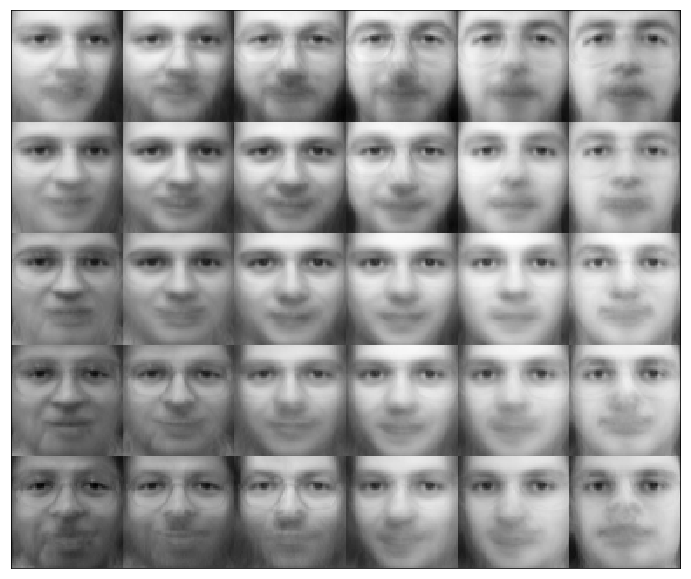
\includegraphics[scale=0.3]{imagenes/facescpu.png}
\caption{Imagen obtenida en el experimento para CPU del mapa auto-organizado.}
\label{img:somcpu}
\end{figure}

\begin{figure}[ht]
\centering
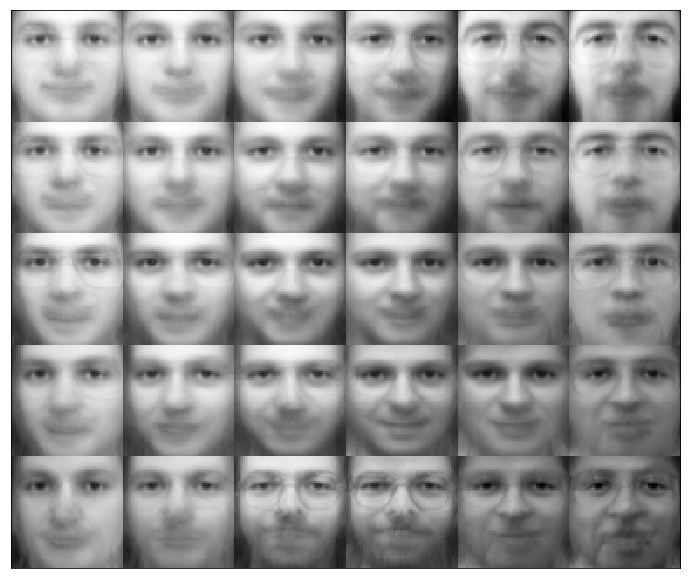
\includegraphics[scale=0.3]{imagenes/facesgpu.png}
\caption{Imagen obtenida en el experimento para GPU del mapa auto-organizado.}
\label{img:somgpu}
\end{figure}

En la figura \ref{img:somcpu}, podemos observar los resultados obtenidos para la ejecución de este algoritmo sobre CPU. En ella, podemos observar que, personas con piel de color más oscuro se agrupan en la esquina superior izquierda, o que, en la fila inferior nos encontramos ante imágenes de la misma persona, donde en las 2 primeras imágenes el sujeto está mirando de lado y, en las siguientes, parece llevar gafas puestas, entre otros detalles. En este ejemplo, obtenemos un error de cuantificación de 6,57 y un error topográfico de 0,0325, tardando un total de 203,09 segundos en su ejecución.\\

En la figura \ref{img:somgpu}, podemos observar los resultados obtenidos para la ejecución de este algoritmo sobre nuestro dispositivo \textit{CUDA}. En ella, podemos observar como, personas que están claramente sonriendo se encuentran en la parte derecha de la penúltima fila, o en la esquina superior derecha, encontramos imágenes del mismo sujeto con gafas puestas. Para este ejemplo, obtenemos un error de cuantificación de 6,56 y un error topográfico de 0,0125, tardando un total de 281,01 segundos en su ejecución.\\
	
En este pequeño experimento, hemos podido comprobar visualmente que ambas implementaciones funcionan correctamente y proporcionan resultados similares, excepto en el tiempo de ejecución, y gran parte de los errores de implementación fueron detectados gracias a este experimento. El hecho de que la versión para GPU tarde más que la versión para CPU a que en cada una de las 10 particiones del \textit{RDD} se evalúan tan sólo 40 muestras y, nuestro algoritmo, en cada iteración y para cada partición, ha de realizar transferencias de memoria entre host y dispositivo, añadiendo un \textit{overhead}. Dado este número bajo de muestras, estamos invirtiendo más tiempo en realizar esas transferencias y lanzar los \textit{kernels} que en los pocos cálculos necesarios. Conforme el número de muestras sea mayor, como veremos en el siguiente experimento, iremos obteniendo mejores resultados con la GPU. 

\subsection{Uso del modelo sobre un conjunto de datos grandes dimensiones.}
Posteriormente, para evaluar la capacidad del algoritmo ante un conjunto de mayores dimensiones, utilizamos SUSY. Para este experimento, ignoramos las etiquetas de salida y utilizamos un mapa de neuronas de 8 filas y 7 columnas con los parámetros de control $\tau$ a 10, $\sigma_0$ a 4, $\sigma_f$ a 0,1. El algoritmo lo ejecutamos durante 10 iteraciones (5 cada fase) y realizamos 4 repeticiones del experimento para tomar una medida de tiempo promedio, con el fin de obtener resultados más fiables que realizando una única ejecución. En este experimento, nos centramos en evaluar como varía el tiempo de ejecución de nuestra implementación y la ganancia conseguida según vamos aumentando el número de muestras totales a evaluar. Nuestro RDD tendrá 10 particiones e iremos variando la cantidad de muestras totales de SUSY que vamos a procesar.

\begin{table}[ht]
\begin{tabular}{@{}l|c|c|c@{}}
\textit{\textbf{Nº de Muestras}} & \multicolumn{1}{l|}{\textit{\textbf{Tiempo CPU (s)}}} & \multicolumn{1}{l|}{\textit{\textbf{Tiempo GPU (s)}}} & \multicolumn{1}{l}{\textit{\textbf{Ganancia}}} \\ \midrule
\textit{\textbf{500000}}         & 231,09                                                & 56,99                                               & 4,06                                          \\
\textit{\textbf{1000000}}        & 426,19                                                & 58,74                                               & 7,26                                           \\
\textit{\textbf{1500000}}        & 618,29                                                & 61,41                                               & 10,07                                           \\
\textit{\textbf{2000000}}        & 822,55                                                & 62,73                                               & 13,11                                           \\
\textit{\textbf{2500000}}        & 1017,45                                               & 66,22                                               & 15,36                                           \\
\textit{\textbf{3000000}}        & 1212,12                                               & 67,75                                               & 17,89                                           \\
\textit{\textbf{3500000}}        & 1398,09                                               & 67,14                                               & 20,83                                           \\
\textit{\textbf{4000000}}        & 1616,68                                               & 67,63                                               & 23,90                                           \\
\textit{\textbf{4500000}}        & 1788,50                                               & 68,45                                               & 26,13                                           \\
\textit{\textbf{5000000}}        & 1992,61                                               & 72,30                                               & 26,99                                          
\end{tabular}
\caption{Tiempos promedios de ejecución y ganancias para el experimento del mapa auto-organizado sobre SUSY.}
\label{tab:susysom}
\end{table}

En la tabla \ref{tab:susysom}, vemos las diferencias entre los tiempos promedios de 4 ejecuciones para CPU y 4 ejecuciones para GPU según los percentiles de muestras propuestos para el experimento. La evolución de los tiempos de ejecución para la GPU oscila en un pequeño intervalo entre los 60-70 segundos (1 minuto). Sin embargo, la evolución de los tiempos para la CPU oscila entre los 231 segundos (casi 4 minutos) y 1992 segundos (33 minutos) por ejecución.  Para una mejor visualización de estos resultados, planteamos la gráfica de la figura \ref{img:somsusy}, en la que combinamos las gráficas de líneas para la evolución de los tiempos promedios con las ganancias obtenidas en una gráfico de barras. \\

\begin{figure}[ht]
\centering
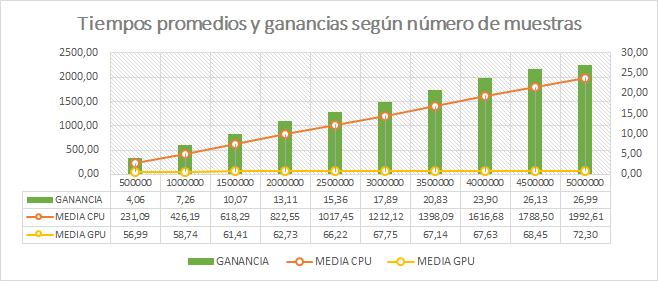
\includegraphics[scale=0.7]{imagenes/susysom.png}
\caption{Gráfica con tiempos promedios y ganancias para SUSY.}
\label{img:somsusy}
\end{figure}

En la gráfica planteada vemos de manera clara cómo, al aumentar el número de muestras, la implementación basada en \textit{CUDA} y \textit{Spark} es considerablemente más rápida que su homóloga para CPU. En el ejemplo más pequeño planteando, es decir, evaluar medio millón de muestras, en el que cada una de las 10 particiones del \textit{RDD} evalúa 50000 muestras, la versión para CUDA es 4 veces más rápida que su homóloga para CPU. En el ejemplo más grande propuesto, es decir, evaluar 5 millones de muestras, el uso de CUDA nos ofrece un tiempo de ejecución casi 27 veces más rápido que la CPU.


\subsection{Resultados de Nsight sobre la versión final del algoritmo.}
Por último, analizamos en profundidad simulamos el entrenamiento del SOM durante una iteración con un ejemplo completamente aleatorio. El total de muestras a evaluar es de 1 millón, divididas en 10 particiones de 100000 muestras. El mapa de neuronas objetivo es de 10 filas por 10 columnas y la dimensión del problema a resolver es de 18 características. En la tabla \ref{tab:profsomkernels}, vemos los tiempos de ejecución de los \textit{kernels} en este experimento.\\

\begin{table}[ht]
\begin{tabular}{@{}|lc|cccc|@{}}
\toprule
                                 & \multicolumn{1}{l|}{}                               & \multicolumn{4}{c|}{\textit{\textbf{Tiempo}}}                                                                                         \\
\textit{\textbf{Kernel}}         & \multicolumn{1}{l|}{\textit{\textbf{Nº usos}}} & \textit{\textbf{mínimo}} & \textit{\textbf{medio}}           & \textit{\textbf{máximo}}          & \textit{\textbf{total}}            \\ \midrule
\textit{\textbf{rand\_weights}}  & 1                                                   & $6,62 \; \mu s$             & $6,62 \; \mu s$                      & $6,62 \;\mu s$                      & $6,62 \;\mu s$                       \\
\textit{\textbf{som\_iter}}      & 10                                                  & $1,61 \; ms$                & $1,835 \; ms$                        & $2,17 \;ms$                         & $18,35 \;ms$                         \\
\textit{\textbf{finish\_update}} & 1                                                   & $37,38 \; \mu s$            & \multicolumn{1}{l}{$37,38\; \mu s$} & \multicolumn{1}{l}{$37,38 \;\mu s$} & \multicolumn{1}{l|}{$37,38 \;\mu s$} \\ \bottomrule
\end{tabular}
\caption{Tiempos de ejecución de los kernels en el experimento de profiling}
\label{tab:profsomkernels}
\end{table}

Como cabía esperar, la mayor parte del tiempo se corresponde a la ejecución del \textit{kernel som\_iter}, que tarda un total de $18,35 \; ms$. El kernel \textit{rand\_weigths} es el más rápido de todos y, aun así, es sólo invocado una vez en el algoritmo, independientemente del número de iteraciones, por lo que no tiene sentido centrarse en optimizarlo mientras se puedan hacer otras mejoras. El kernel \textit{finish\_update}, que será llamado tantas veces como iteraciones se realicen en el algoritmo ocupan el puesto intermedio, siendo 49 veces más rápido que una llamada al \textit{kernel som\_iter}. Además, el \textit{kernel som\_iter}, siempre será llamado las mismas veces que \textit{finish\_update} multiplicado por el número de particiones del \textit{RDD} por lo que, a ser posible, hemos de centrarnos en mejorar este \textit{kernel}.\\

\begin{figure}[ht]
\centering
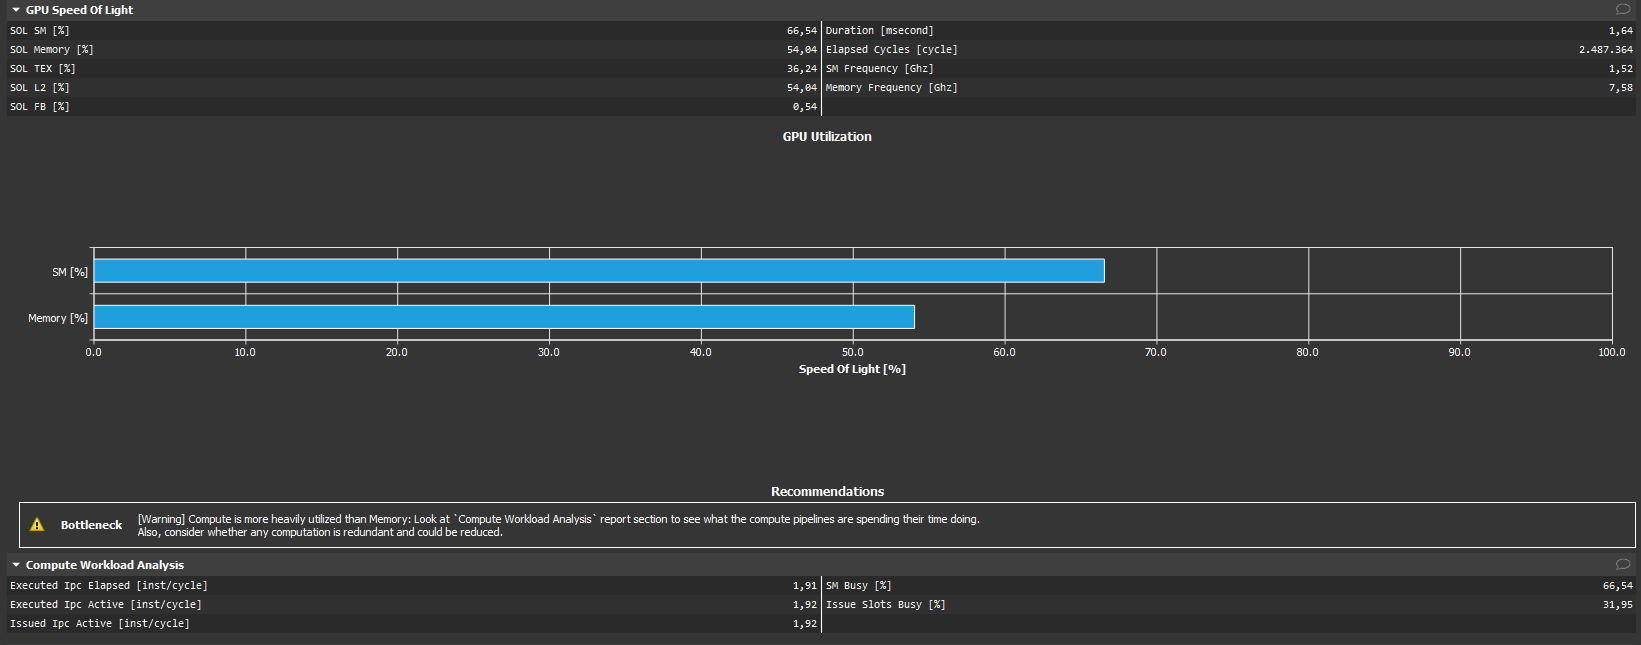
\includegraphics[scale=0.3]{imagenes/som_sol.png}
\caption{Speed of Light del kernel evaluado.}
\label{img:sol}
\end{figure}

Un análisis más profundo del \textit{kernel som\_iter} con el profiler nos revela que, el cuello de botella ,se debe a los cálculos realizados (figura \ref{img:sol}). La medida \textit{``Speed Of Light (SOL)''} nos indica lo cerca que estamos de alcanzar el rendimiento teórico máximo de unidades de \textit{hardware} durante la utilización del dispositivo CUDA en el \textit{kernel}. Podemos observar que, en nuestro caso, estamos aprovechando un 66,54 \% de la capacidad máxima de computación de nuestra GTX 1060.\\

\begin{figure}[ht]
\centering
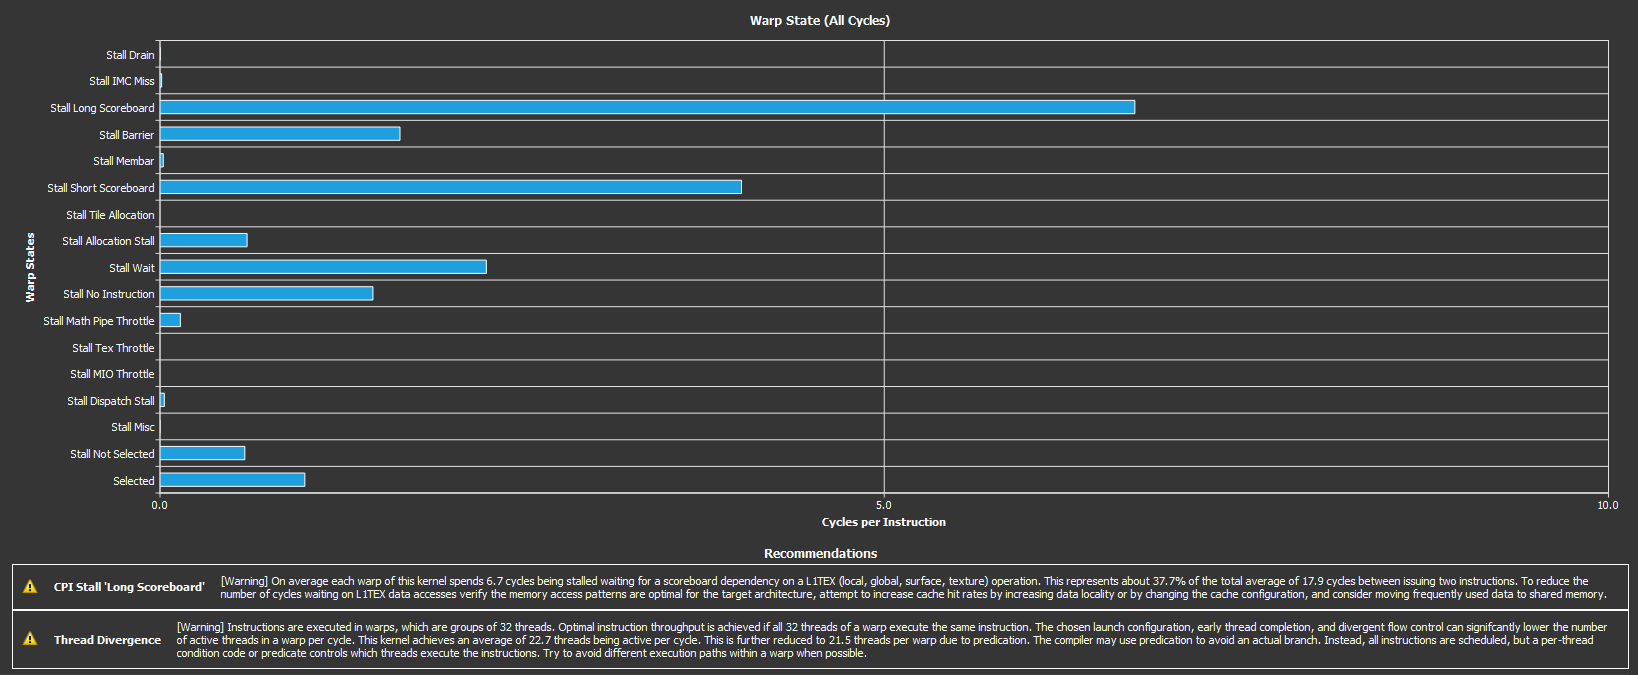
\includegraphics[scale=0.3]{imagenes/som_warp_states.png}
\caption{Análisis de los warps del kernel.}
\label{img:warpssom}
\end{figure}

En la figura \ref{img:warpssom} vemos las dos razones principales que hacen que el \textit{kernel} no funcione más rápido. Una de ellas es la cantidad de accesos a memoria dentro del dispositivo y la otra es la divergencia de las hebras, es decir, situaciones en las que las hebras quieren ejecutar diferentes instrucciones.\\

 Todos los elementos dentro de un bloque que eran utilizados más de una vez fueron cargados en memoria compartida, por lo que, podemos intuir que este problema radica de conflictos que surjan del uso de las operaciones de suma atómica. Encontrar una alternativa mejor que la planteada para el cálculo de los pesos parciales debería de ser la prioridad a la hora de optimizar este algoritmo. \\

 Por otro lado, el segundo problema que destacamos es la divergencia, que se debe principalmente a que, en este ejemplo, trabajamos con 128 hebras por bloque mientras que el número de neuronas es 100, por lo que uno de los \textit{warps} utilizará tan sólo 4 de las 32 hebras. En un caso ideal, el tamaño del mapa tendría un número de neuronas que fuese potencia de 2 (al menos 32). Si tuviésemos garantizado que esto fuese a ocurrir, podríamos eliminar gran parte de los condicionales utilizados, ya que, no sería necesario comprobar si hay más hebras que neuronas, ni habría que rellenar distancias extras con infinito, ni tendríamos que realizar todas las comprobaciones en la reducción para tamaños de bloque superiores al número de neuronas.

\section{Experimentos para evaluar el random forest.}
Para la evaluación de los resultados del \textit{random forest}, hemos utilizado el conjunto de datos SUSY. Para entrenar el \textit{random forest}, se ha usado validación cruzada con 10 iteraciones, es decir, el conjunto de muestras se ha dividido en 10 subconjuntos de muestras del mismo tamaño; en cada iteración, 9 de esos subconjuntos han sido utilizados para entrenar el \textit{random forest} y uno para evaluar los resultados; y, para finalizar, se ha realizado un promedio de los resultados. Para evaluar el modelo, hemos utilizado tres métricas: precisión, que indica el porcentaje de muestras que han sido correctamente clasificadas; el tiempo que tarda en entrenar el algoritmo; y la ganancia de la GPU a la CPU, o sea, cuántas veces es más rápida la tarjeta gráfica que el procesador. \\

Puesto que, tanto la versión para GPU como para CPU utilizan el mismo algoritmo pero, adaptado para las correspondientes arquitecturas, la precisión es un factor relevante a la hora de comprobar si la implementación de los algoritmos es correcta, ya que, en caso de una buena implementación, independientemente de haber usado GPU o CPU, obtendríamos precisiones idénticas, y estos resultados podemos compararlos con los obtenidos en aproximaciones similares en la literatura. \\

Además, durante el proceso de implementación, hemos utilizado otros conjuntos de datos, como Spambase \cite{spambase} o \textit{MAGIC} \cite{magic04}, para comprobar los resultados mientras utilizábamos un único árbol, cuyos resultados podemos ver en la siguiente tablas:

\begin{table}[H]
\centering
\begin{tabular}{@{}|c|cc|cc|@{}}
\toprule
\textbf{\begin{tabular}[c]{@{}c@{}}SPAMBASE\\ 4601 muestras\\ 57 atributos\end{tabular}} & \multicolumn{1}{c|}{\textit{\textbf{GPU}}} & \textit{\textbf{\begin{tabular}[c]{@{}c@{}}CPU \\ (1 core)\end{tabular}}} & \multicolumn{1}{c|}{\textit{\textbf{GPU}}} & \textit{\textbf{\begin{tabular}[c]{@{}c@{}}CPU\\ (1 core)\end{tabular}}} \\ \midrule
\textit{\textbf{Profundidad}}                                                            & \multicolumn{2}{c|}{\textit{\textbf{Tiempo (s)}}}                                                                      & \multicolumn{2}{c|}{\textit{\textbf{Precisión (\%)}}}                                                                 \\ \midrule
\textbf{4}                                                                               & 0,06                                       & 0,19                                                                      & 87,77                                      & 87,77                                                                    \\
\textbf{5}                                                                               & 0,1                                        & 0,24                                                                      & 89,65                                      & 89,65                                                                    \\
\textbf{6}                                                                               & 0,14                                       & 0,32                                                                      & 91,04                                      & 91,04                                                                    \\
\textbf{7}                                                                               & 0,21                                       & 0,42                                                                      & 91,82                                      & 91,82                                                                    \\
\textbf{8}                                                                               & 0,3                                        & 0,55                                                                      & 92,11                                      & 92,11                                                                    \\ \bottomrule
\end{tabular}
\caption{Resultados de evaluar un árbol de decisión con validación cruzada con 10 iteraciones en SPAMBASE}
\label{tab:spambase}
\end{table}

\begin{table}[H]
\centering
\begin{tabular}{@{}|c|cc|cc|@{}}
\toprule
\textbf{\begin{tabular}[c]{@{}c@{}}MAGIC04\\ 19020 muestras\\ 10 atributos)\end{tabular}} & \multicolumn{1}{c|}{\textit{\textbf{GPU}}} & \textit{\textbf{\begin{tabular}[c]{@{}c@{}}CPU\\ (1 core)\end{tabular}}} & \multicolumn{1}{c|}{\textit{\textbf{GPU}}} & \textit{\textbf{\begin{tabular}[c]{@{}c@{}}CPU\\ (1 core)\end{tabular}}} \\ \midrule
\textit{\textbf{Profundidad}}                                                             & \multicolumn{2}{c|}{\textit{\textbf{Tiempo (s)}}}                                                                     & \multicolumn{2}{c|}{\textit{\textbf{Precisión (\%)}}}                                                                 \\ \midrule
\textbf{4}                                                                                & 0,05                                       & 0,25                                                                     & 79,1                                    & 79,1                                                               \\
\textbf{5}                                                                                & 0,1                                        & 0,35                                                                     & 81,99                                   & 81,99                                                               \\
\textbf{6}                                                                                & 0,17                                       & 0,48                                                                     & 82,94                                   & 82,94                                                              \\
\textbf{7}                                                                                & 0,31                                       & 0,68                                                                     & 84,07                                   & 84,07                                                                 \\
\textbf{8}                                                                                & 0,55                                       & 0,98                                                                     & 84,42                                   & 84,42                                                                  \\ \bottomrule
\end{tabular}
\caption{Resultados de evaluar un árbol de decisión con validación cruzada con 10 iteraciones en MAGIC04.}
\label{tab:magic04}
\end{table}

En ambas tablas podemos observar cómo la precisión obtenida en la versión para CPU como la versión para GPU es idéntica, garantizándonos que al menos ambas implementaciones, aunque hayan sido adaptadas para sus arquitecturas correspondientes, proporcionan los mismos resultados. Su elevado porcentaje de precisión, que se parecen a los obtenidos por aproximaciones similares presentes en la literatura llevan a pensar que la implementación es correcta. Por otro lado, aunque hayamos anotado el tiempo de ejecución en este experimento como referencia durante el proceso de desarrollo, hemos de recalcar que estamos comparando una versión del algoritmo en CUDA con una versión secuencial en la que sólo se utiliza uno de los núcleos de la CPU, por lo que es normal que los tiempos de entrenamiento requeridos en la GPU sean inferiores a los que la CPU ha necesitado.\\

Para la evaluación del \textit{random forest} con \textit{SUSY} hemos generado un \textit{random forest} con 12 árboles y hemos utilizado validación cruzada con 10 iteraciones sobre el total de los 5 millones de muestras disponibles en el conjunto de datos. El experimento ha sido realizado múltiples veces, variando la profundidad de 4 a 10. Además, el experimento ha sido repetido 5 veces, anotando los resultados promedios, que podemos observar en la tabla \ref{tab:rf}.\\
\begin{table}[ht]
\centering
\begin{tabular}{@{}l|ll|c|c|@{}}
\cmidrule(l){2-5}
\textit{\textbf{}}                                  & \multicolumn{1}{l|}{\textit{\textbf{GPU}}} & \textit{\textbf{CPU}} & \multicolumn{1}{l|}{\textit{\textbf{GPU vs CPU}}} & \multicolumn{1}{l|}{\textbf{GPU/CPU}} \\ \midrule
\multicolumn{1}{|c|}{\textit{\textbf{Profundidad}}} & \multicolumn{2}{c|}{\textit{\textbf{Tiempo (s)}}}                  & \textit{\textbf{Ganancia}}                        & \textbf{Precisión (\%)}               \\ \midrule
\multicolumn{1}{|l|}{4}                             & 25,58                                      & 27,64                 & 1,08                                              & 75,82                                 \\
\multicolumn{1}{|l|}{5}                             & 26,06                                      & 31,71                 & 1,22                                              & 76,99                                 \\
\multicolumn{1}{|l|}{6}                             & 26,20                                      & 35,30                 & 1,35                                              & 77,44                                 \\
\multicolumn{1}{|l|}{7}                             & 26,45                                      & 38,19                 & 1,44                                              & 78,33                                 \\
\multicolumn{1}{|l|}{8}                             & 27,34                                      & 40,87                 & 1,49                                              & 78,67                                 \\
\multicolumn{1}{|l|}{9}                             & 29,97                                      & 45,85                 & 1,53                                              & 79,02                                 \\
\multicolumn{1}{|l|}{10}                            & 33,63                                      & 48,66                 & 1,45                                              & 79,25                                 \\ \bottomrule
\end{tabular}
\caption{Resultados de Random Forest para SUSY con 12 árboles}
\label{tab:rf}
\end{table}

A diferencia del mapa auto-organizado, podemos observar que, en este caso, los resultados en este modelo se encuentran mucho más ajustados. Para poder realizar una interpretación adecuada de los tiempos de ejecución y la ganancia, hemos de tener en cuenta los siguientes factores:

\begin{itemize}
	\item Dada la implementación realizada, la versión para GPU conseguirá mejores resultados conforme mayor sea el número de elementos a procesar.
	\item El número de árboles utilizados en el \textit{random forest} va a influir en el tiempo de ejecución de la GPU. Conforme mayor sea el número de árboles utilizados, menor será el tamaño de elementos que tenemos garantizados que se procesen a la vez, si estamos usando una única GPU.
	\item Árboles muy profundos afectan de manera negativa a la GPU, debido a que, conforme pasemos al siguiente nivel de profundidad, vamos a tener un mayor número de nodos con un menor número de muestras cada uno o incluso parte de las muestras habrían sido eliminadas en alguna poda, que, limitando la capacidad de aprovechar la máxima capacidad de paralelismo posible.
\end{itemize}

En el ejemplo mostrado en la tabla \ref{tab:rf}, observamos que la versión para GPU nos ofrece una mejora del tiempo de ejecución al usar la GPU. En la profundidad 4, obtenemos el resultado que menos mejora nos ofrece con una diferencia de tan sólo 2 segundos. Mientras que la cantidad de datos sea lo suficientemente grande, una mayor profundidad implica más procesamiento de datos y vamos a obtener una mejor ganancia hasta la profundidad 9, en la que obtenemos la mejor ganancia, siendo la versión para GPU 1,53 veces más rápida que la correspondiente para CPU dándonos una ventaja de 15,88 segundos. En la profundidad 10, observamos cómo esa ganancia empieza a decaer bajando a 1,45 veces más rápido. \\

En el caso de la precisión, una mayor profundidad nos ayuda a obtener mejores resultados, partiendo de un 75,82 \% en la profundidad 4 hasta un 79,25 \% en la profundidad 10. . En comparación con otras aproximaciones de la literatura utilizadas para resolver este problema, la implementación realizada queda considerablemente por detrás del 85-87 \% obtenido utilizado otros modelos \cite{susy}. \\

Para concluir este análisis, podemos determinar que varios factores van a influir en qué situaciones va a ser mejor nuestra aproximación.
\begin{itemize}
\item Para considerar utilizar este modelo hemos de estar trabajando con bases de datos de una combinación de número de muestras y número de atributos considerablemente grandes.
\item El número de árboles utilizados va a influir tanto en la precisión como en el tiempo de ejecución. Por regla generar, un mayor número de árboles va a mejorar la precisión pero va a reducir la velocidad de entrenamiento si se va a utilizar una única GPU. En el caso de disponer de un clúster, tener un número de GPUs igual al número de árboles nos permitiría obtener los mejores resultados, siempre y cuando el tiempo de comunicación entre los nodos del clúster no sea demasiado alto.
\item Dependiendo del problema a resolver podremos variar el número de árboles o la profundidad que queremos usar para entrenar. Como veíamos antes, para casos más pequeños, como \textit{Spambase} o \textit{MAGIC04}, en los que utilizábamos un único árbol obteníamos resultandos competentes con la literatura en términos de precisión (92,11 \% para Spambase y 84,42 \% para MAGIC04, utilizando árboles de profundidad 8 en ambos casos).
\end{itemize}

\subsection{Resultados del uso del profiler sobre la versión final del algoritmo.}
En el caso del árbol de decisión desarrollado, el principal cuello de botella es la necesidad de lanzar una gran cantidad de \textit{kernels} muy rápidos que no hemos sido capaces de compactar para evitar el \textit{overhead} de cada lanzamiento de un kernel. Para evitarlo, hemos utilizado algunas técnicas para evitar este problema como el uso de \textit{streams} concurrentes o la combinación de múltiples \textit{kernels} (scan con cálculo del criterio de Gini y scan con el cálculo de las nuevas posiciones en la lista de atributos). Cabe también destacar, que otra alternativa a evaluar para solucionar este problema es el uso del paralelismo dinámico de \textit{CUDA}, que permite lanzar un kernel desde otro, sin embargo, no tenemos acceso a esa característica usando \textit{Python}.\\

Puesto que hay una alta variedad de \textit{kernels}, que son invocados frecuentemente, vamos a observar la siguiente gráfica, en la que vemos el porcentaje del tiempo de ejecución que se dedica a cada tarea en una reproducción del experimento, con una base de datos de 100000 muestras aleatorias con 18 atributos y generando un árbol de profundidad 10.

\begin{figure}[ht]
\centering
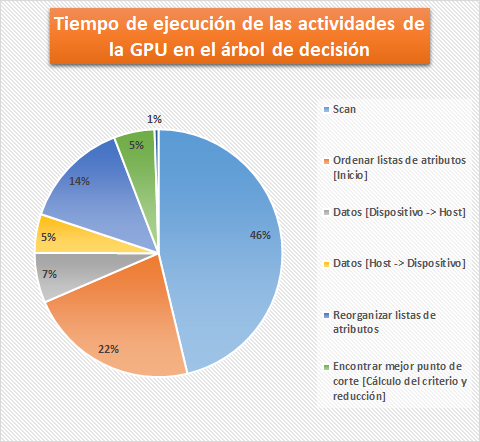
\includegraphics[scale=0.8]{imagenes/profiletreequesito.png}
\caption{Análisis de los kernels ejecutados.}
\label{img:quesito}
\end{figure}

En primer lugar, la operación que más porcentaje de tiempo lleva es la operación más costosa, la organización de la listas de atributos inicial que toma un 27 \% del tiempo total de ejecución de la GPU, correspondiente al algoritmo de ordenación de CuPy. Esta operación, que junto a la inicialización de la lista de atributos supone el inicio del algoritmo, acumulado un 29 \% del tiempo usado. Una posible vía de mejora es evaluar si una implementación propia del algoritmo de ordenación nos proporcionaría resultados mejores. En caso de realizar una implementación propia, podríamos combinar con facilidad la inicialización de las listas de atributos con el algoritmo de ordenación. \\

En segundo lugar, tenemos un empate al 20 \% entre la reducción utilizada para calcular el criterio de Gini y la reorganización de la listas de atributos. La operación de reducción es invocada para todos los nodos activos mientras que la reorganización de atributos es realizada una vez por nivel de profundidad. \\

La implementación de la reducción para este algoritmo sigue una estructura similar a la operación de \textit{scan}. Ésta, hace uso de operaciones intrínsecas de \textit{warps} y de operaciones atómicas para calcular el mínimo global entre los bloques. Otra alternativa probada fue el lanzamiento de otro kernel para el cálculo de los resultados globales, pero resultó ligeramente más lenta que el uso de las operaciones atómicas. Otra opción a evaluar, sería el uso del paralelismo dinámico, pero como comentamos previamente, no podemos acceder a esa característica desde \textit{Numba}.\\

La reorganización de la listas de atributos es una operación de transferencia de memoria dentro del dispositivo. En primer lugar, los datos son movidos a \textit{arrays} temporales y, una vez finalizado el proceso, se sobrescriben los datos en las nuevas posiciones. Dentro del dispositivo \textit{CUDA}, estas transferencias de memoria son considerablemente rápidas, especialmente cuando los datos siguen algún patrón de adyacencia, como sucede al rellenar los arrays temporales. Sin embargo, en el caso de los accesos a memoria aleatorios, como ocurre en la fase de escritura, el tiempo de acceso va a ser mucho más lento, que queda manifestado en que, de ese 20 \%, un 5,1 \% se corresponde a la primera fase y el resto a la segunda. \\

Por último, vamos a analizar las tres operaciones relacionadas con la primitiva de \textit{scan}, que son las siguientes en la gráfica. La operación de \textit{scan} es usada dos veces por nodo activo, una primera vez para calcular el criterio de Gini y, una segunda vez, para calcular qué transferencias de memoria permiten mantener el orden de los atributos sin tener que volver a usar el algoritmo de ordenación, haciendo de ella la operación que es invocada el mayor número de veces por ejecución del algoritmo. A diferencia del caso de la reducción, en vez de utilizar operaciones atómicas, usamos el lanzamiento de un nuevo \textit{kernel} para realizar el cálculo global del \textit{scan}. Este cambio se debe a que, dadas las necesidades de lanzar otros \textit{kernels} para ejecutar el algoritmo sin paralelismo dinámico hemos podido combinar el cálculo del \textit{scan} global con la operación posterior. La parte que realiza el cálculo de la primitiva \textit{scan} para cada bloque representa un 15 \% del tiempo de ejecución de la GPU mientras que el \textit{kernel} que termina la primitiva y calcula el criterio de Gini conlleva un 8 \% del tiempo y el cálculo de los nuevas posiciones para ordenar un 5 \%. Puesto que, ambos \textit{kernels} parten de la misma operación (realizar el \textit{scan} global) podemos deducir que la complejidad aritmética del cálculo del criterio de Gini es superior a la del cálculo de las nuevas posiciones.\\

Aunque el análisis previo nos facilita saber qué \textit{kernel} nos interesaría optimizar primero es importante observar un resultado más genérico obtenido en el \textit{profile} nos indica que durante los 0,25 segundos que ha tardado en entrenarse el árbol sólo 0,1 segundos han sido usados para realizar los cálculos, proporcionado un porcentaje de utilización de la GPU del 40 \%. Este problema deriva principalmente del \textit{overhead} de tener que lanzar múltiples \textit{kernels}, que viene dada por la necesidad de evaluar múltiples nodos independientes, que, además, han de ser sincronizados al terminar cada nivel de profundidad para reorganizar las listas de atributos y poder pasar al siguiente nivel.